\chapter{Botnet Economics and Business Models}
\markboth{Botnet Economics and Business Models}{}
\chaptauthors{Famos Tobias, Mannhart Thomas, Tham David, Waltert Gian }

\Kurzfassung{%
This is the abstract.
It fits pretty much on one page and is definitely not longer.}

\newpage

\minitoc %table of contents

\newpage

\section{Introduction}

\subsection{Motivation}
Online Crime has shifted in the last 20 years. Where earlier attacks and malicious actions were performed by individual hackers, trying to break things mostly for fun there are now organised groups build like companies that act as malicious actors in the cyber space. (Copy some of economics of online crime introduction)
Cybercrime is a field of high revenue. It is estimate that the global revenue from cybercrime is at least 1.5 Trillion Us Dollars [5]. In context, that would be roughly equivalent to the GDP of Australia in the year 2018. [6]
The Damage done by cybercrime is estimated to have risen about 12\% from 2017 to 2018 [1] and in total numbers estimated to be 600 Billion US Dollars [4]. 

Some of the currently big threats in the cyber security landscape are coupled to Botnets, a network of computers controlled by attackers (Putman et al Business). Botnets can be used for various malicious intents and actions such as Distributed Denial of Services Attacks, Spam Generation, Information Theft and data exfiltration. 
There is an increasing number of devices connected to the internet every day. Furthermore, there are predictions that there will be 75 Billion IoT devices in the world by the year of 2025. 
And many of them are poorly secured, if at all. This leads to a serious incentive for Botnet providers to target not only personal computers and smartphones, but also IoT devices such as security cameras, washing machines or doorbells. Devastating examples of the abuse of vulnerabilities in IoT devices, such as default or hardcoded credential can be found in mass. Huge botnets like Linux. Aidra, Mirai or Bashlite infect tens of thousands of devices and use them for malicious purposes.   
The high number of Devices connected to the internet, paired with the trend for more bandwidth and manifacturing devices with more CPU power and better Network cards to output higher bandwidths gives malicious actors more possibilities to abuse foreign infrastructure and devices. 
Additionally there is a lack of incentives for Device Owners to secure their devices, since there is no direct, perceptible impact from an insecure device onto them, or so they think. 

\subsection{Malware in numbers}
As the revenue from cybercrime is growing, the development of malware is too. Researchers estimate, that there are 300000 to 1Million new Viruses developed every day [4] Currently, the fastest growing malware thread is ransomware [4]. The FBI estimates that there are more than 4000 ransomware attacks preformed every day, with 209 Million US Dollars Ransom payed in the first quarter of 2016. This is a rapid growth compared to the 24 Million Dollars in ransom payment in the whole year 2015. 
The deployment of Malware onto personal Computers is also changing and growing. The Symantec Threat report states that the primary delivery of Malware has changed in recent years, from malicious URLs to Malicious attachments. From the Malicious attachments, 48 \% are Office Files with Macros used to download Malware. 
A interesting rise in the cyber crime landscape is the mobile ransomware. These malware target mobile devices, and lock them down. [7]
Furthermore the threads concerning IoT devices are equally rising. Symantec has seen an increase in internet of things attacks in the year 2017 and the attack numbers stabilising in the year 2018 [7]. The most attacked devices in their IoT honeypot were routers and security cameras. Together they accounted for 90\% of the IoT attacks, with routers having 75\% and security cameras at 15\% [7]. In terms of protocols was Telnet the mostly used one with 90\% of attempted attacks being done using it in 2018. This is up from50\% in the year 2017 [7]. 
In terms of threads, the top three accounted for over 75\% of the attacks on the IoT honeypots. Namely they were Linux.Lightaidra, Linux.Kaiten and Linux.Mirai. Thus the Mirai Botnet still is an active thread with 15\% of attacks originating in it. [7] 
Overall one can state, that Phishing is still the most popular and easiest way to commit a cybercrime. Due to the low costs of Phishing and the perceived low risk of getting caught phishing remains an attractive attack vector.[4]

 
\subsection{Organisation / Outline}
In the following Paper, we want to show the importance of further research about Botnets and the importance of Botnets itself. By giving a brief overview about the topic of Botnets and their possible usage we want to add to the awareness of the reader about the dangers of botnets and the importance of the influence of botnets on the economy. This is underlined by applying the stated analysis and facts onto a botnet in the case study. 


		
\section{Background}
	\subsection{Botnet}
		\subsubsection{Definition}
			A botnet is a network of infected end-hosts called bots (also referred to as zombies or drones) under the control of a botmaster. Botnets recruit vulnerable machines using basic methods of malware distribution. The botmaster is the manager of the botnet and controls his bots by using command and control (C\&C) channels. These channels are used by the botmaster to distribute his commands to his bots. These channels can use multiple communication mechanisms like P2P or Internet Relay Chat (IRC). A vast majority are using IRC [1].
			
		\subsubsection{Malware}
Malware stands for malicious software and describes any software that is designed to damage or exploit the infected machine. In our case, the malware is the code installed on the vulnerable machine, that turns it into a bot and allows the botmaster to take control.
Malware spreads using multiple techniques and one specific malware can use more than one of these.

A virus is a malicious piece of code that hides inside a host program. It replicates itself when the host program is executed and inserts its own code into other programs.

Worms are standalone programs that replicate and spread themselves when introduced to a computer network.

The name Trojan horse or Trojan describes any malware, that hide their true and malicious intent. This can be a seemingly useful program, an unsuspicious e-mail attachment or an interesting advertisement.


		\subsubsection{Revenue Models}
In today's botnet economy, the attacker using a botnet is rarely the creator and botmaster of the used botnet. Botnets are traded and rented, to generate revenue without performing attacks [2]. There already exist services for development, distribution and hosting of botnets. In many cases, this even includes customer support. Bottazi and Me (2014) call this model Cybercrime-as-a-Service (CaaS) [3].

With Distributed Denial-of-Service (DDoS) attacks revenue can be generated by executing attacks on competitors in the market and getting a part of their market share or executing attacks on behalf of a competitor in exchange for payment.
Another possibility is cyber extortion, by threatening a DDoS attack if a certain amount of money is not paid to the attacker.

Theft and fraud: Botnets are responsible for the majority of spam distributed through the internet (i.e. phishing mail). They are used to host fake websites (phishing websites) to steal personal and valuable information and they enable click fraud [4]. Click fraud is the exploitation of pay-per-click online advertising by imitating a real user and clicking on the advertiser's link. The advertiser has to pay the publisher and the advertising network, therefore creating a potential conflict of interest.

		\subsubsection{Command and Control}
Command and control channels (C\&Cs) are used to communicate with the bots in a botnet. Those channels are based on basic internet communication protocols. The majority of known botnets are using C\&Cs based on the IRC (Internet Relay Chat) protocol. The botmaster can send and receive massages to and from his bots through a centralized command and control mechanism. The communication is in real-time and is highly successful. There are known botnets using the HTTP protocol for their C\&C. This approach is still centralized but the botmaster cannot directly interact with his bots. The bots have to contact the C\&C server to get their commands [5].

		\subsubsection{Architecture}
The architecture refers to the model of communication between the botmaster and his bots. We divide these models into three categories: centralized, decentralized, hybrid and unstructured.

In the centralized model (Figure \ref{fig:centralized}), there is one (or few) central point(s) responsible for the exchange of commands and data between the botmaster and his bots. This central point is the C\&C server and runs on a machine with a high bandwidth connection. This server runs a communication service (mostly IRC). This model provides a small latency which makes it easy to control the botnet. A disadvantage of this model is the high vulnerability of the botnet communication. because this central point is responsible for the whole C\&C communication. If this central point gets discovered and eliminated, it renders the whole botnet useless. This threat can be reduced by using multiple redundant servers controlling the same botnet [6].

\begin{figure}[ht]
\begin{center} 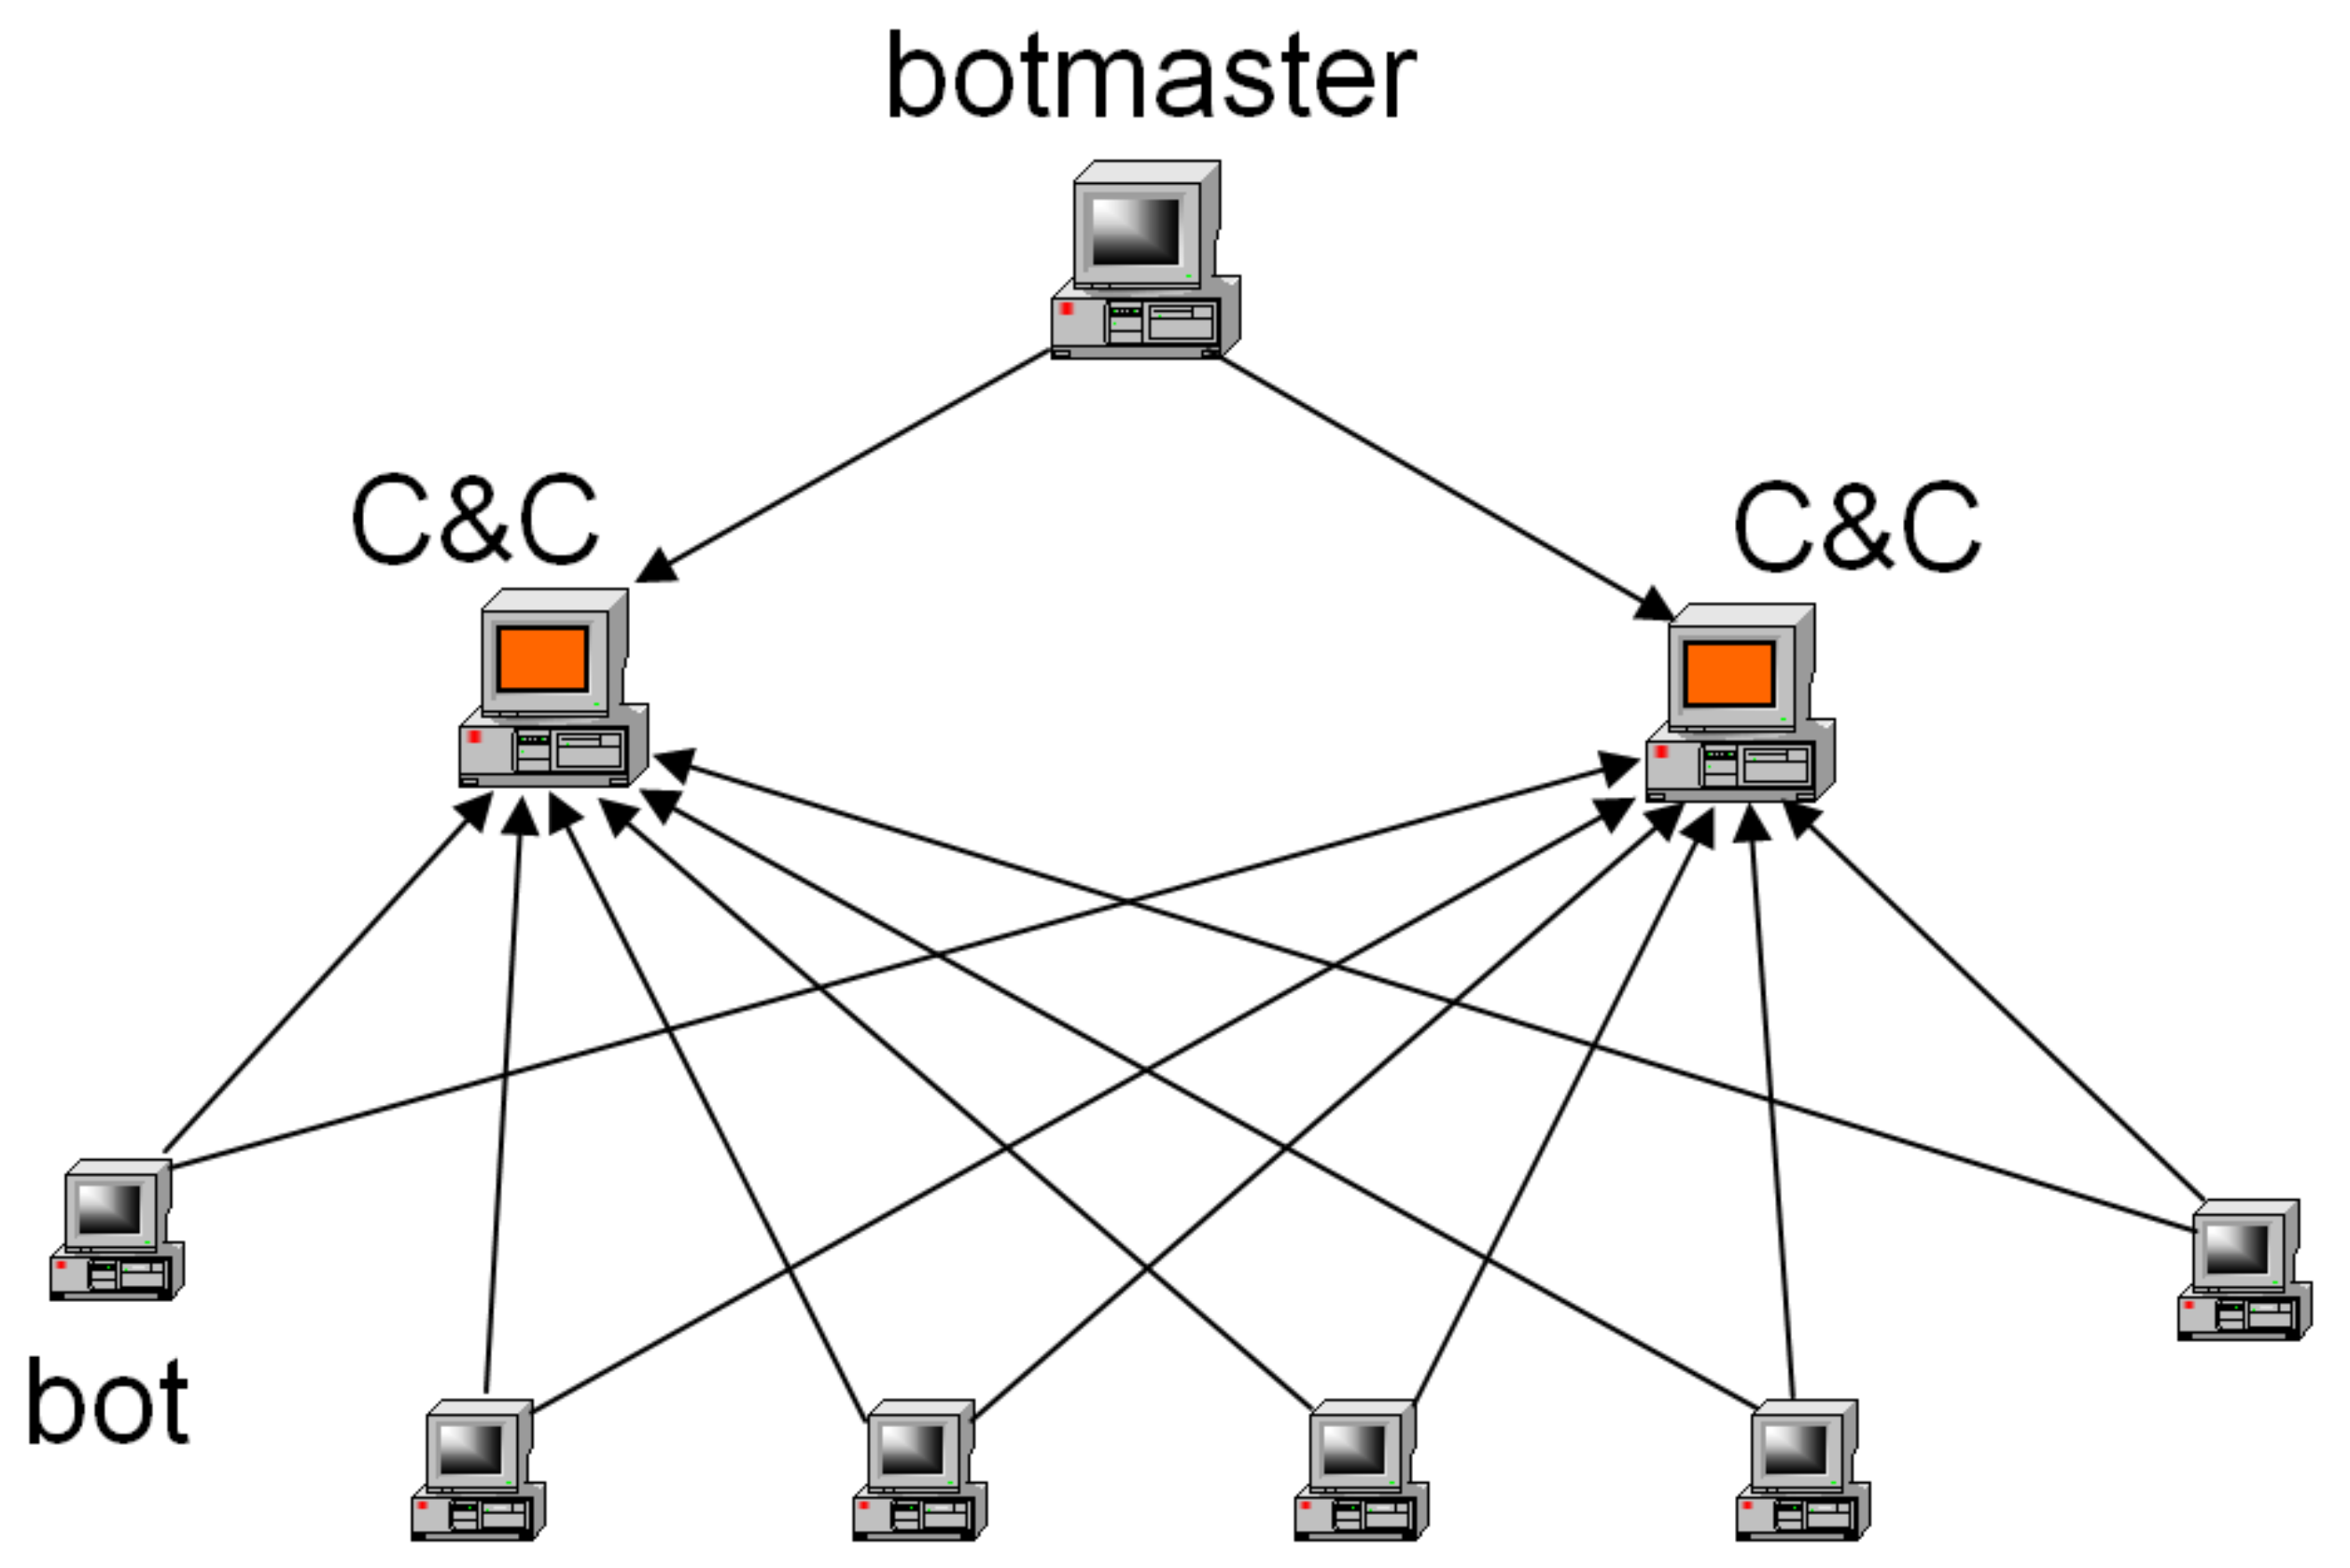
\includegraphics[scale=0.3]{Talk11/CC-centralized} \end{center}
\caption{Command and control architecture of a Centralized model. \textit{Quelle: Zeidanloo and Manaf (2009)}}
\label{fig:centralized}
\end{figure}

The decentralized model (Figure \ref{fig:decentralized}) is a way to eliminate the vulnerabilities of the centralized approach. By using a P2P pattern for C\&C, the system no longer depends on a few selected servers. The bots are interconnected and function as host and as server simultaneously. Each bot knows a fraction of the botnet to send and receive the commands of the botmaster. So even if some bots are detected and taken down, the rest of the botnet continues to receive commands. Zeidanloo and Manaf (2009) stated, that the use of P2P based communication in botnets will be used dramatically in the near future, because botnets using this form of communication are much more challenging to detect and destroy [6].

\begin{figure}[ht]
\begin{center} 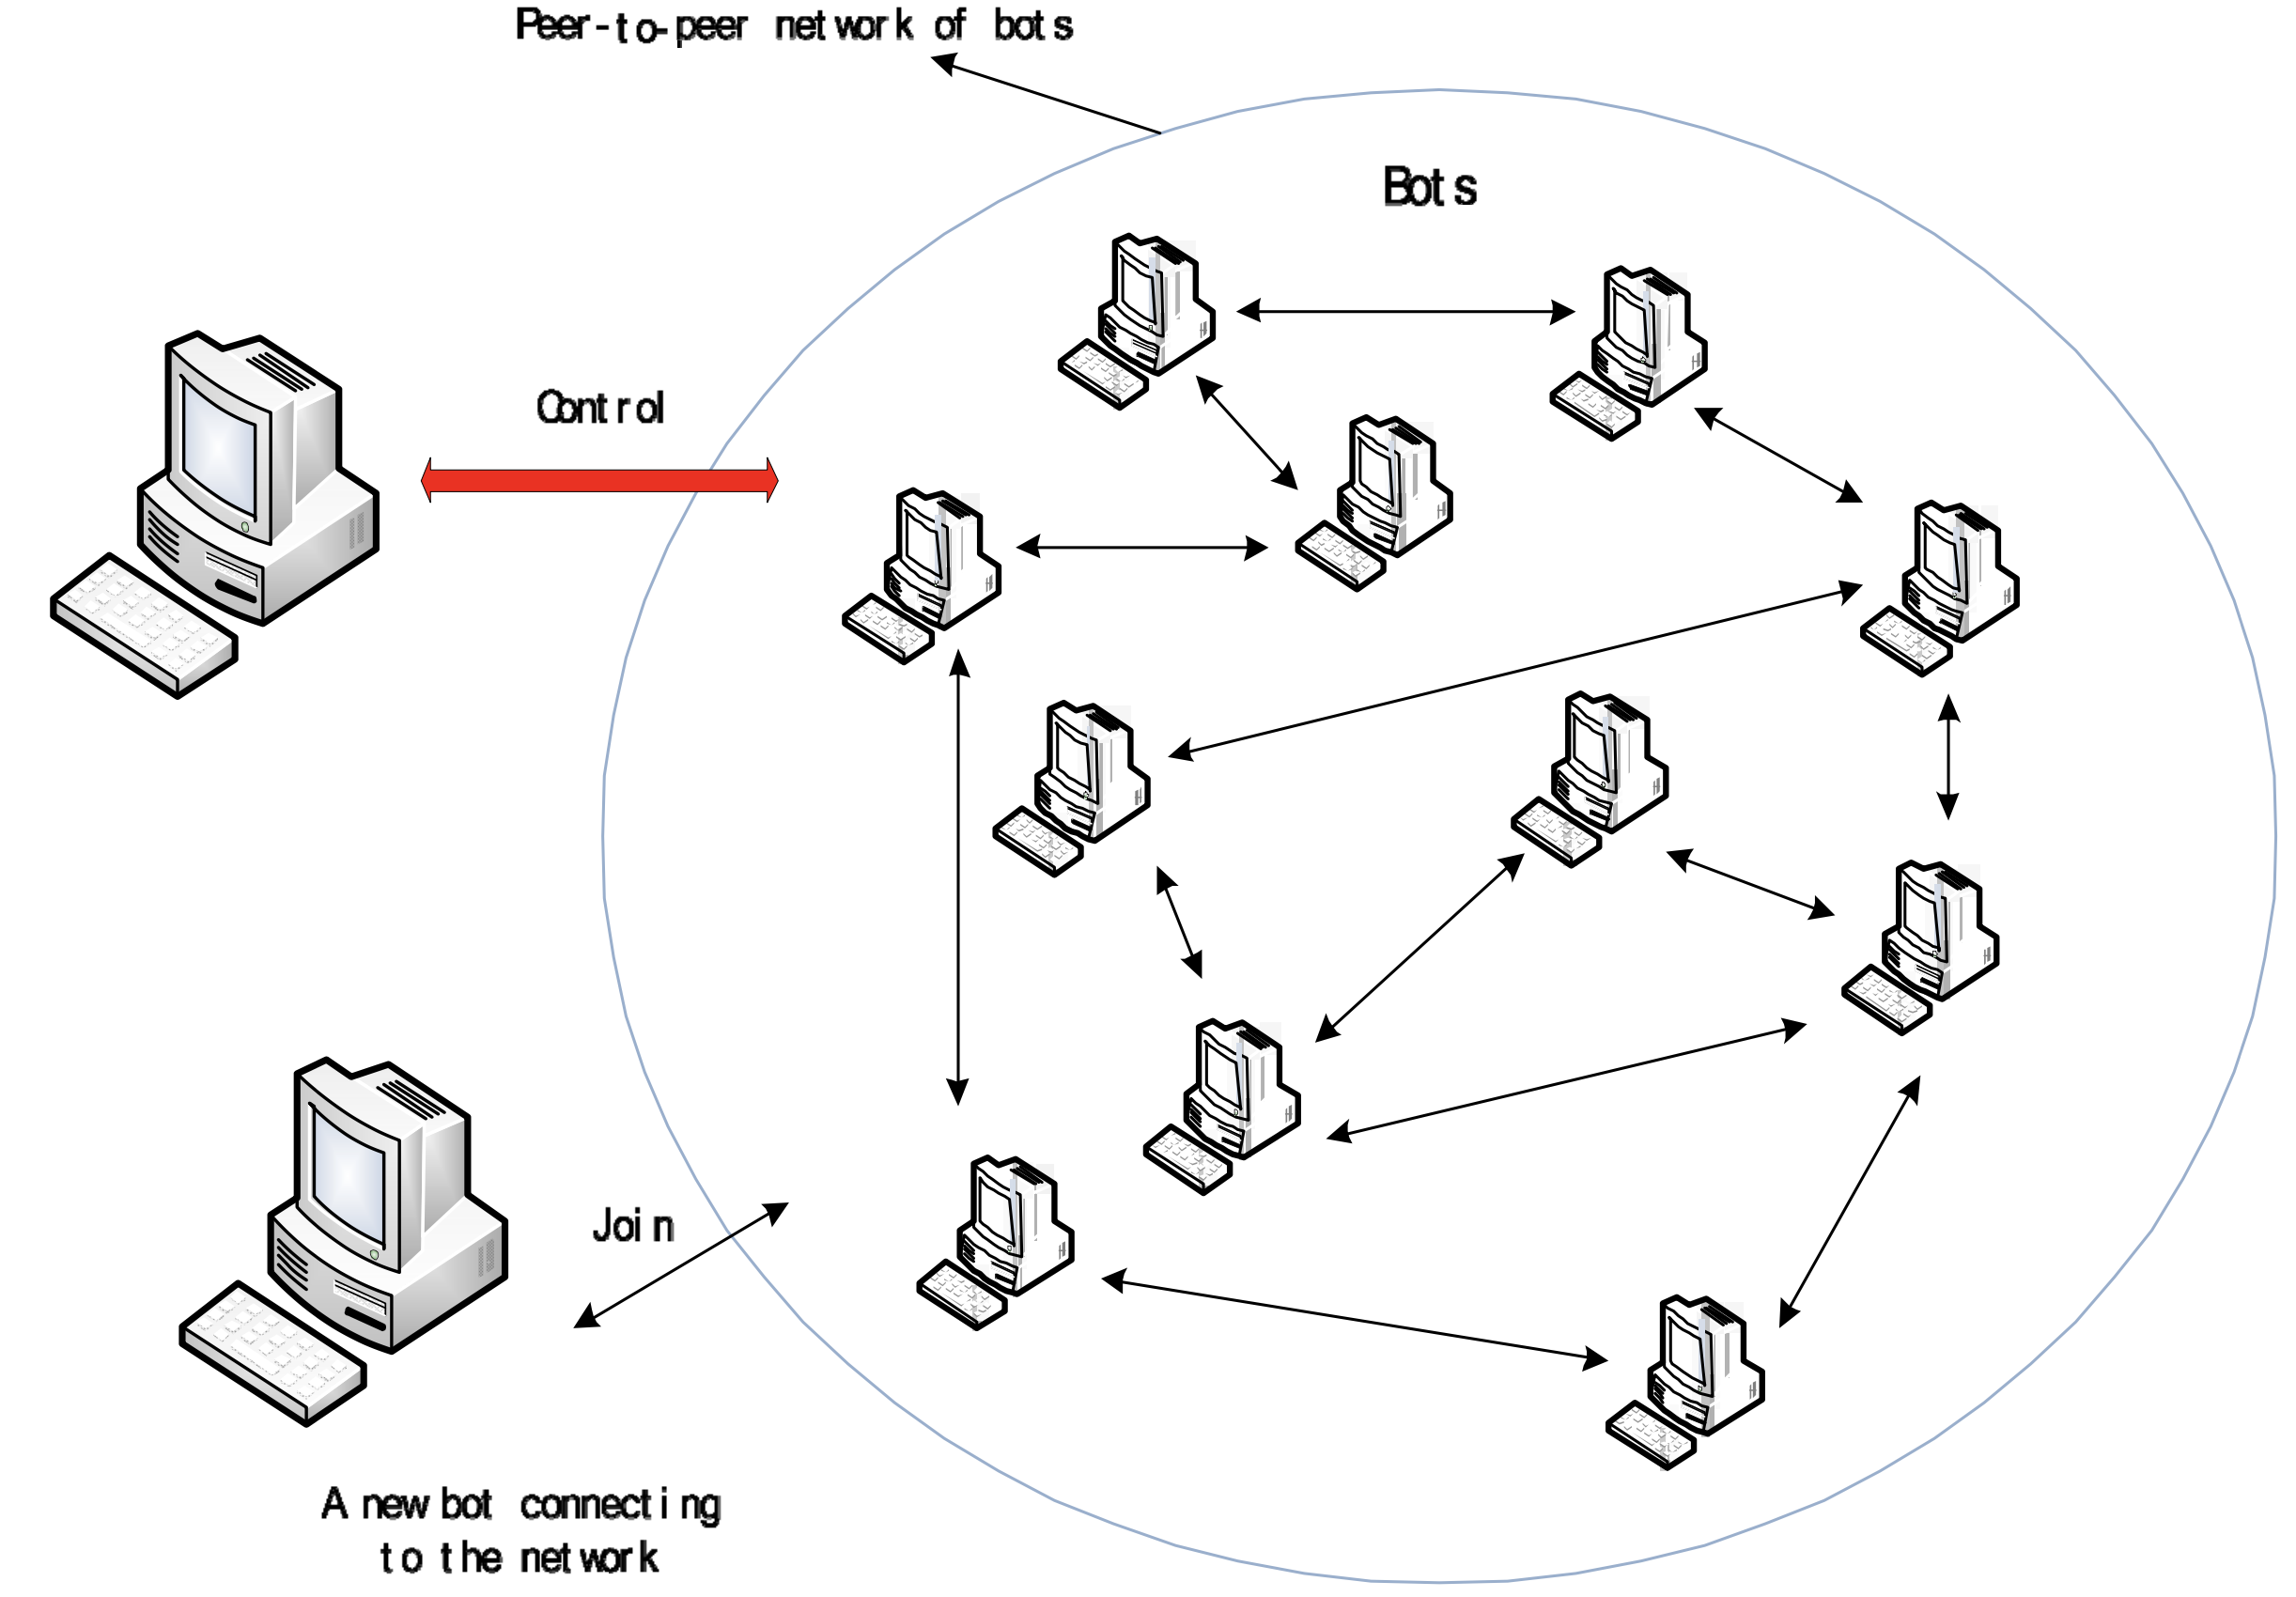
\includegraphics[scale=0.3]{Talk11/CC-P2P} \end{center}
\caption{Example of Peer-to-peer Botnet Architecture. \textit{Quelle: Zeidanloo and Manaf (2009)}}
\label{fig:decentralized}
\end{figure}

Wang et al. (2010) proposed a hybrid model (Figure \ref{fig:hybrid}) that uses the best of both worlds. Such a botnet would contain two types of bots. The Servant Bots, which serve as clients and hosts have static and routable IP addresses. These Servant Bots are accessible from the whole internet, which means they are not behind a firewall that restricts incoming traffic. The Client Bots do not accept incoming connections and have a peer list containing only Servant Bots. The Client bots connect regularly to the Servant Bots in their peer list and forward any new commands to the whole list [7].

\begin{figure}[ht]
\begin{center} 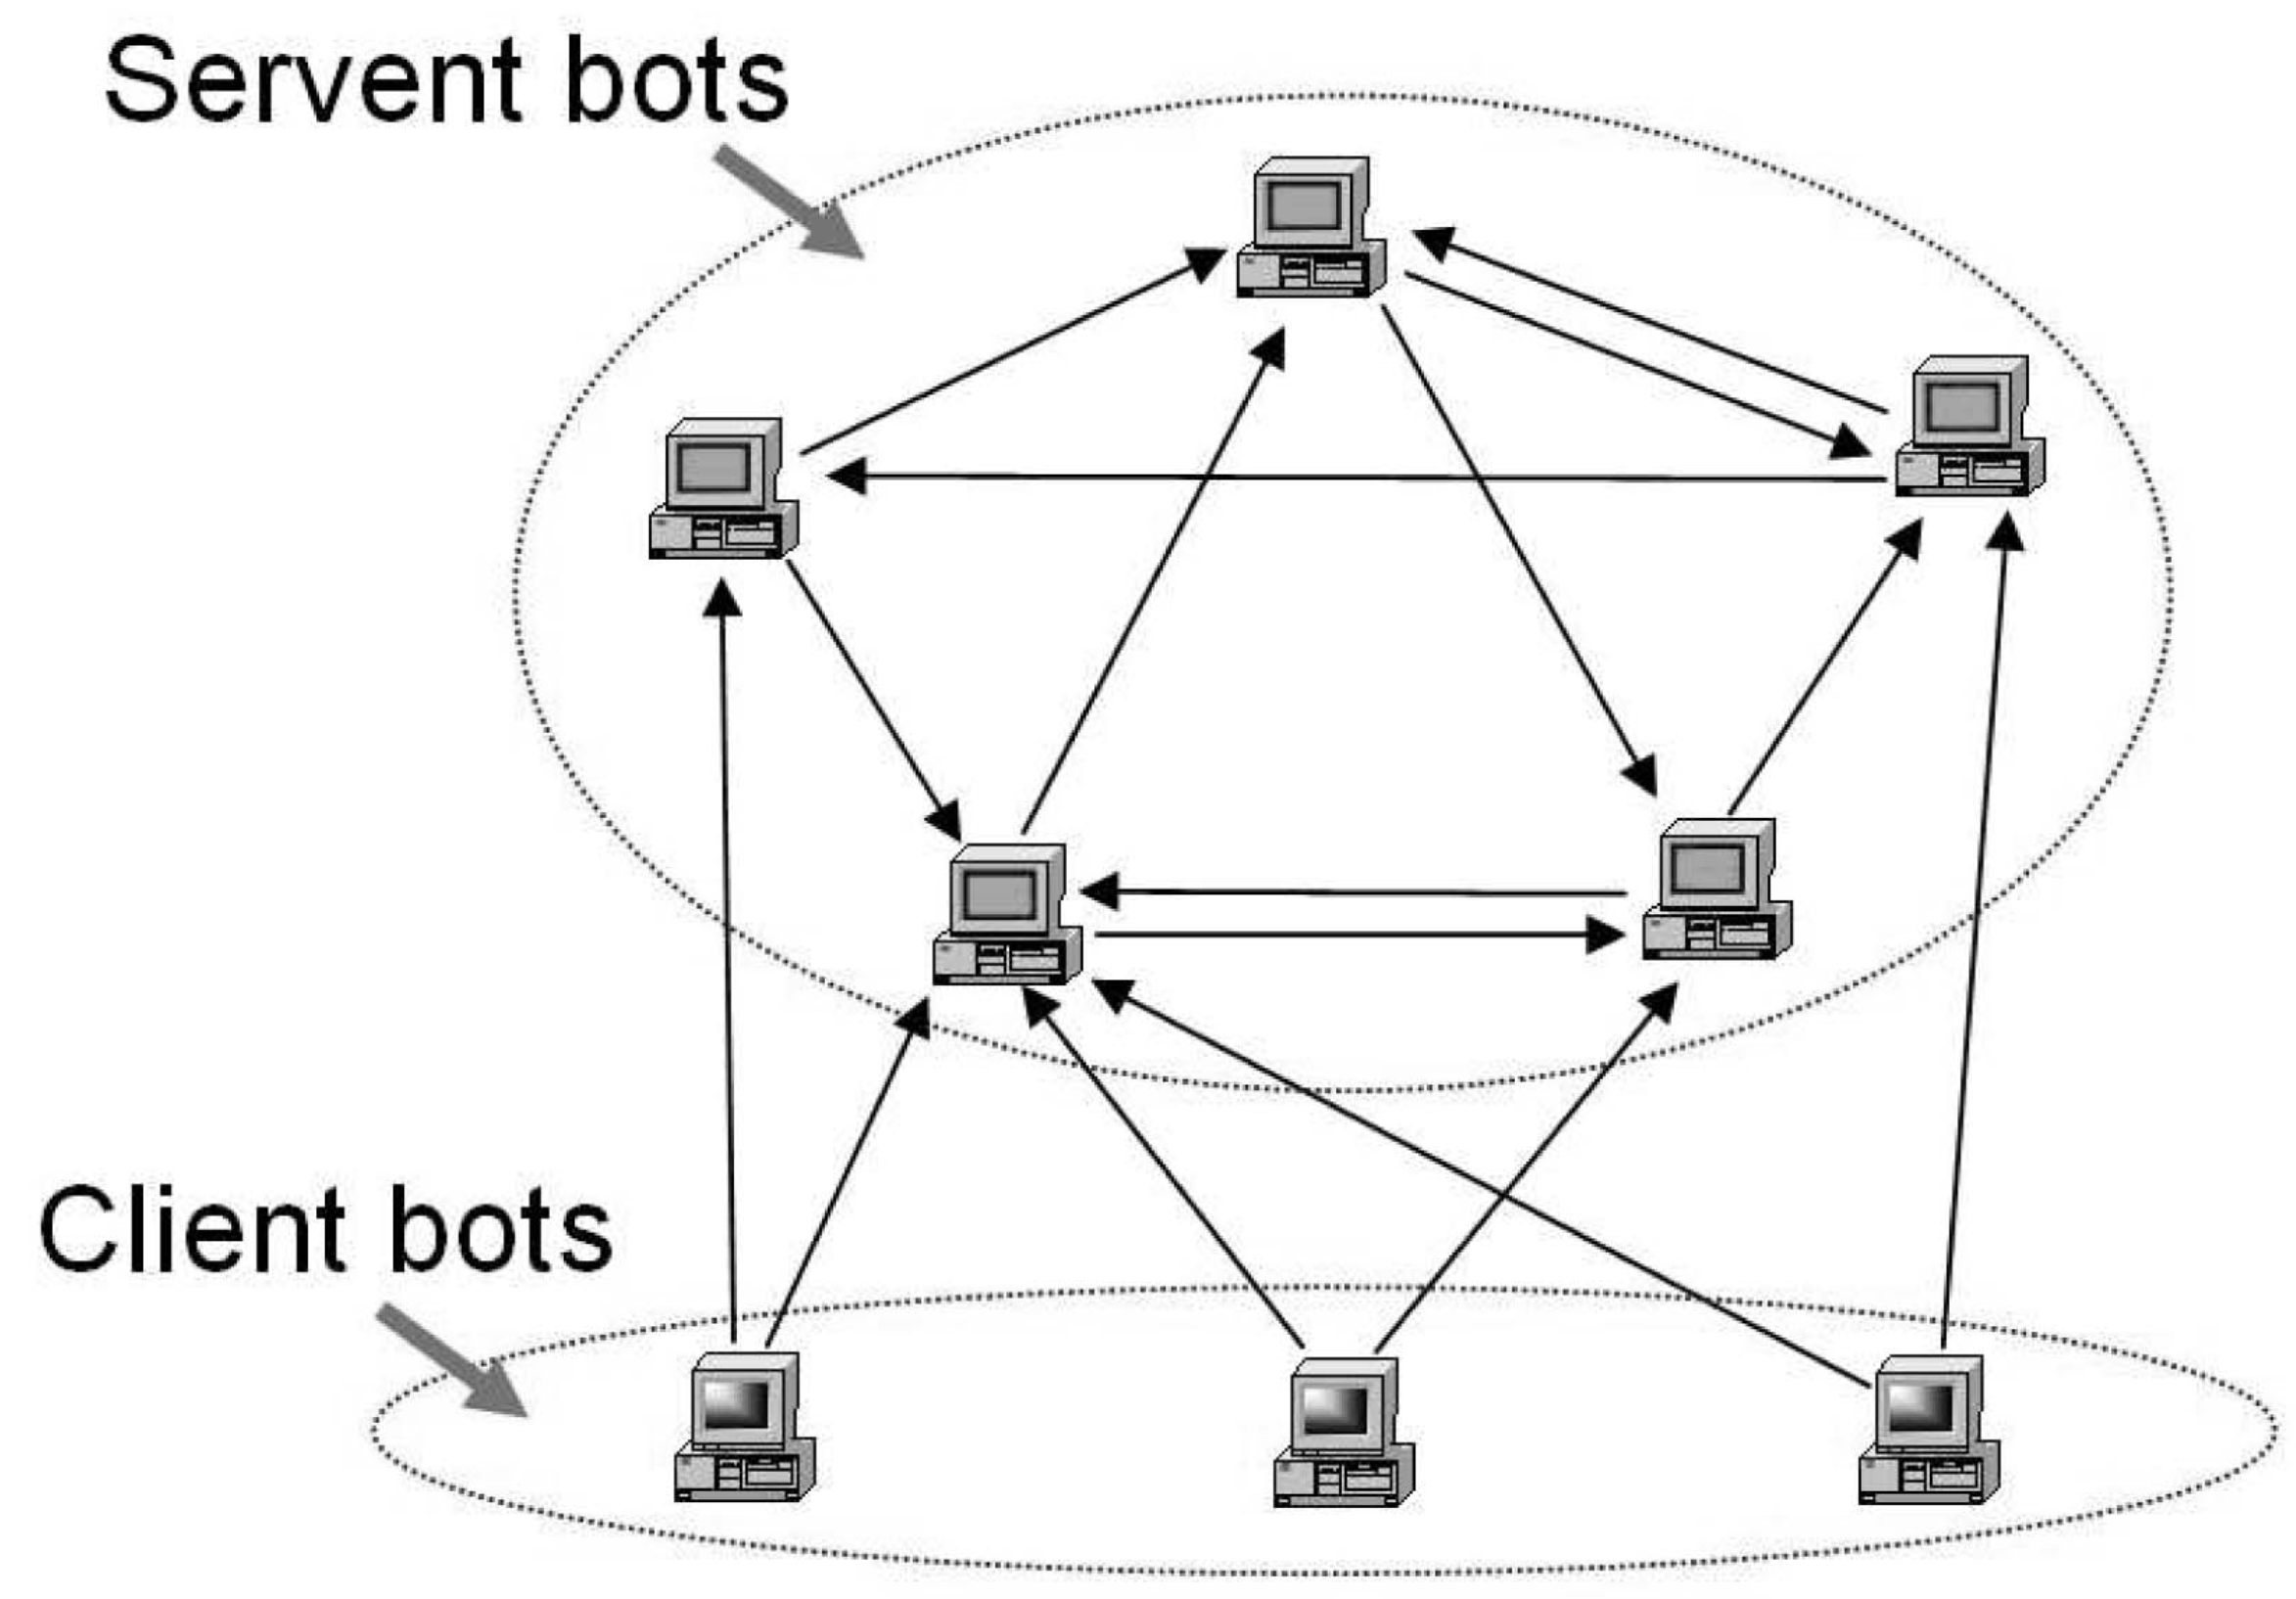
\includegraphics[scale=0.3]{Talk11/CC-hybrid} \end{center}
\caption{C\&C architecture of the proposed hybrid P2P botnet. \textit{Quelle: Wang et al. (2010)}}
\label{fig:hybrid}
\end{figure}

An unstructured communication model is based on the principle, that if a bot receives a command from the botmaster, it randomly scans the internet for other bots to propagate the massage. In this case the rest of the botnet will not be affected if a bot gets discovered. The drawbacks are an extremely high latency, the noticeable scanning and that it cannot be guaranteed, that every bot in the botnet receives the command [8].

		\subsubsection{Underground Markets}
As Thomas et al. (2006) state in their article, that there are entire IRC networks dedicated to cybercrime. Those IRC servers are not hidden, but easy to find and easily accessible. The participants in these underground networks often use encryption to hide their identity.
Most of these networks have channels for helping new members and reporting fraud. Members known to have committed fraud are recorded and shared on the network as a form of self-policing.
There are also other such underground networks using HTTP, Instant Massaging, Peer-to-Peer (P2P) and other forms of communication [*].

		\subsubsection{Distributed Denial-of-Service Attacks (DDoS)}
A Denial-of-Service (DoS) attack attempts to prevent the legitimate use of a service by either overwhelming the service with a huge amount of traffic or exploiting an application or protocol by sending malformed packages and causing the service to freeze or reboot. A Denial-of-Service (DoS) attack becomes a Distributed Denial-of-Service (DDoS) attack, if the source of the attack are multiple distributed entities or rather bots in a botnet (Figure \ref{fig:ddos}) [9].

\begin{figure}[ht]
\begin{center} 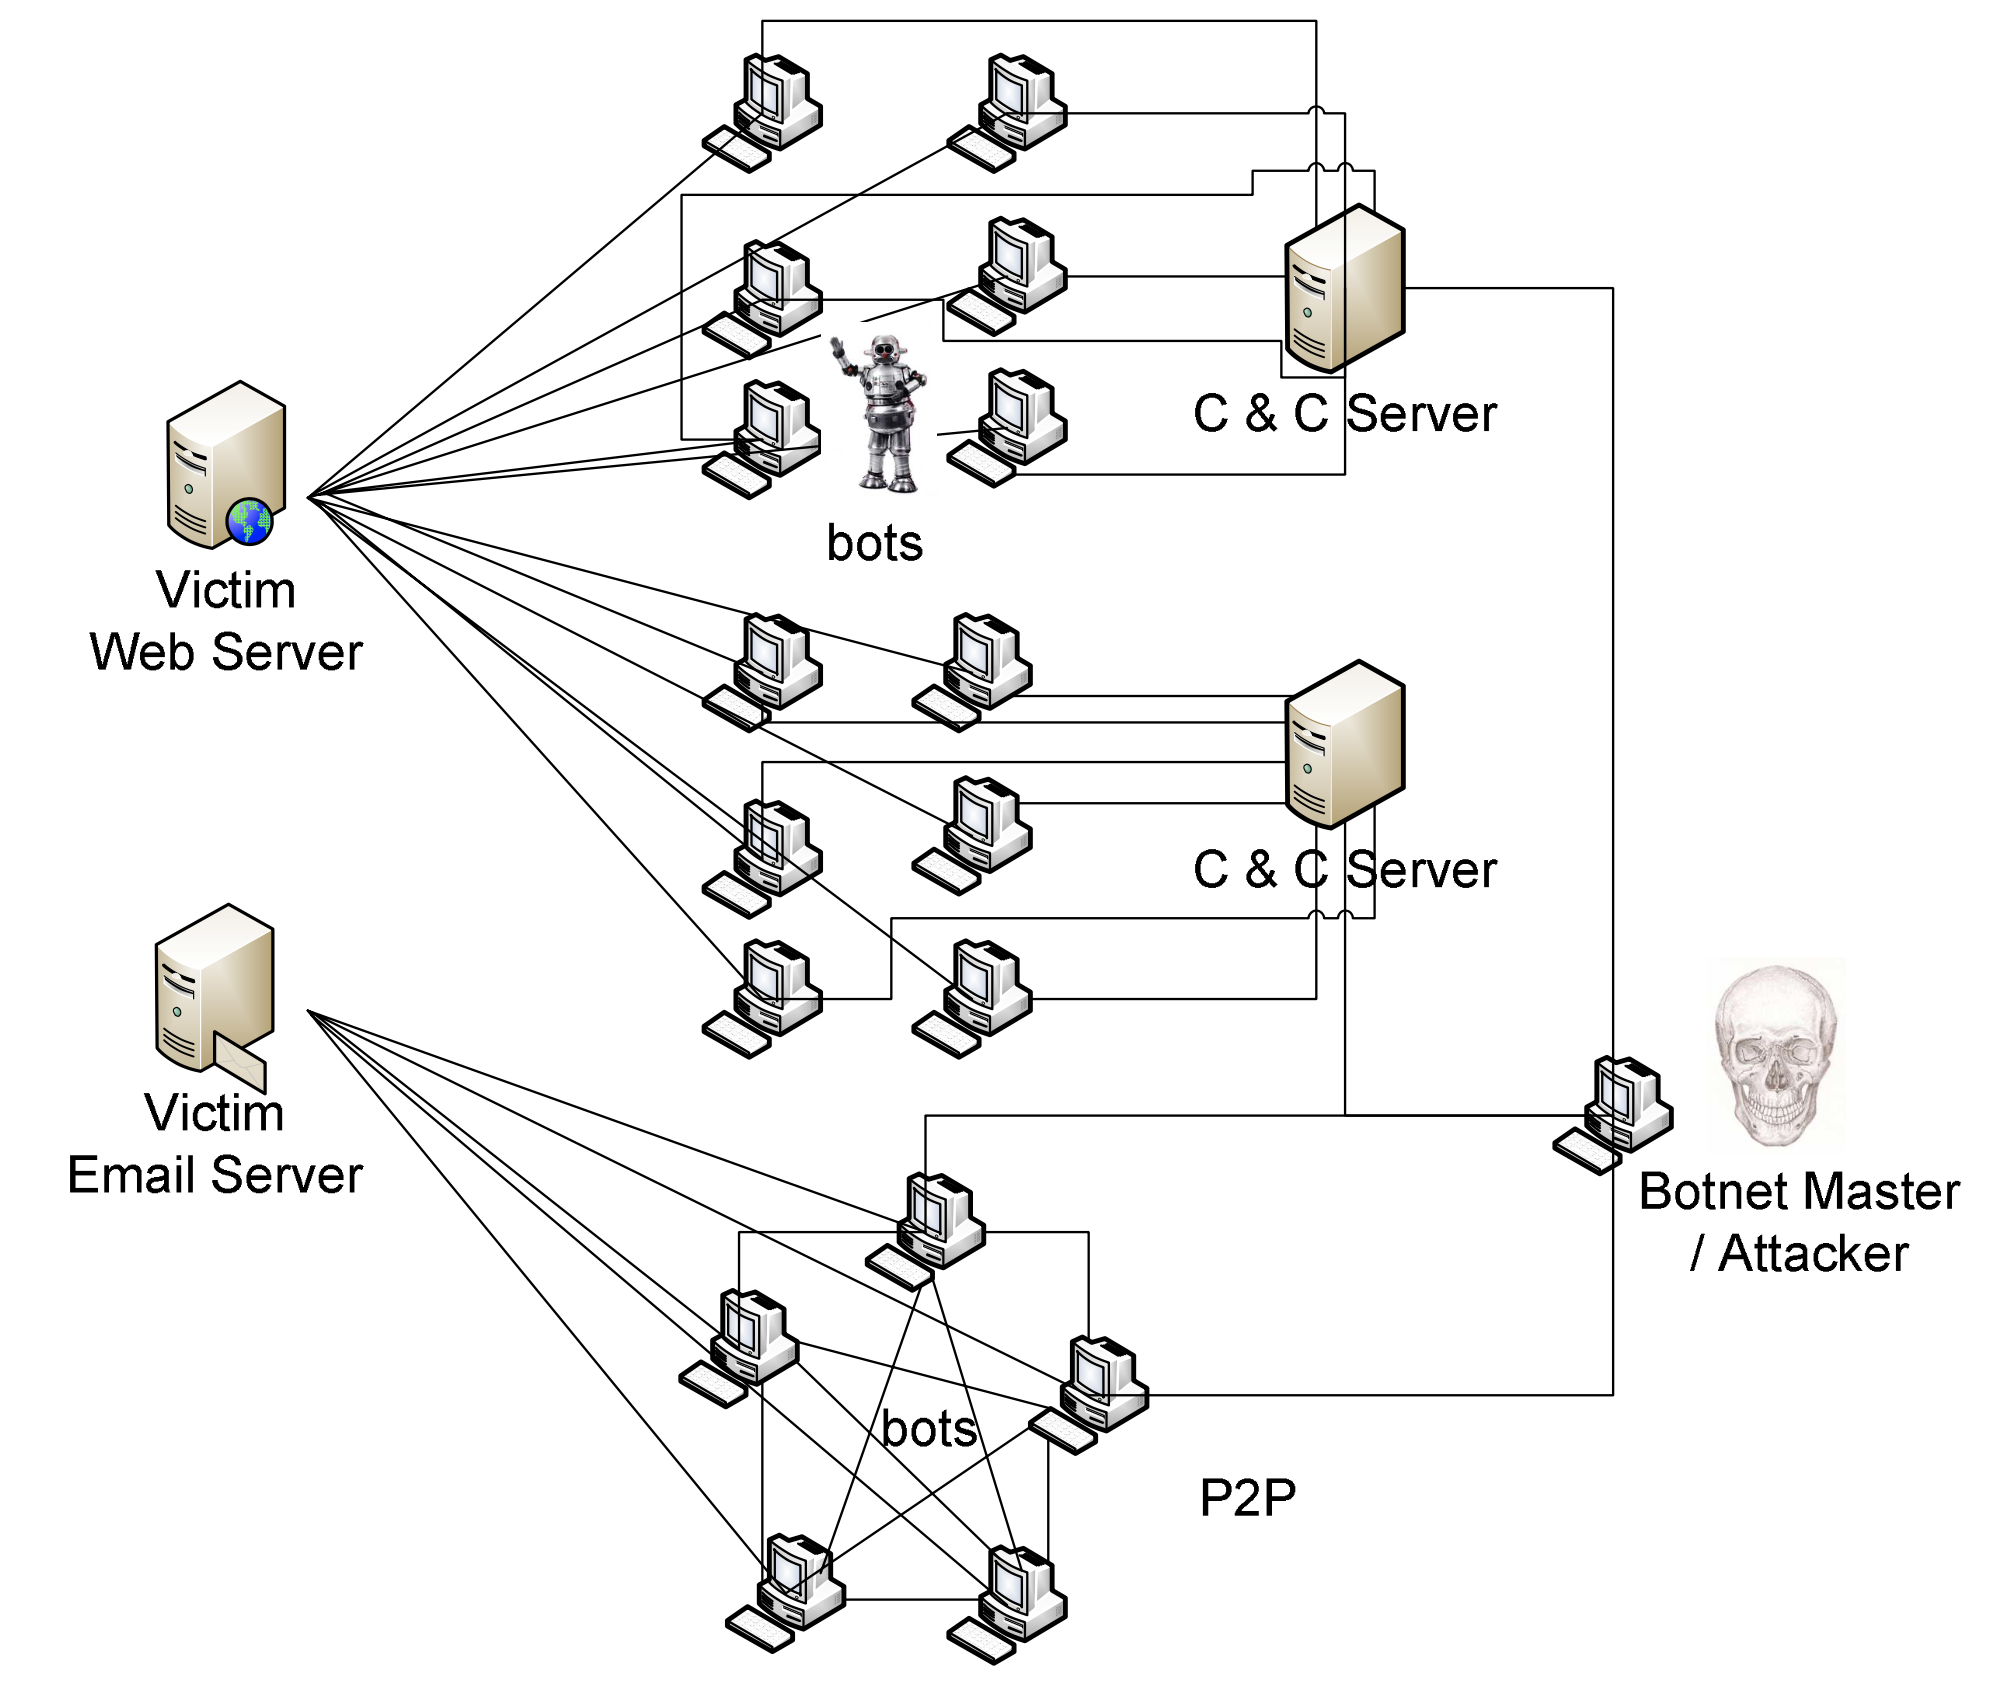
\includegraphics[scale=0.4]{Talk11/DDoS-attack} \end{center}
\caption{A scenario of botnet attacks launched by robot computers (bots) controlled by the botnet master and attacker. \textit{Quelle: Li et al. (2009)}}
\label{fig:ddos}
\end{figure}

An increasingly popular form of DDoS attacks are DDoS amplification attacks, like the memcached DDoS attack on GitHub on February 28, 2018. The attacker abused memcached instances to amplify the attack by up to 51'000 times the originally sent data. The memcached's response has been targeted to addresses used by GitHub.com using IP address spoofing. This amplification resulted in a peak of 1.35Tbps via 126.9 million packets per second sent to GitHub's services (Figure \ref{fig:ddos}) [10].

\begin{figure}[ht]
\begin{center} 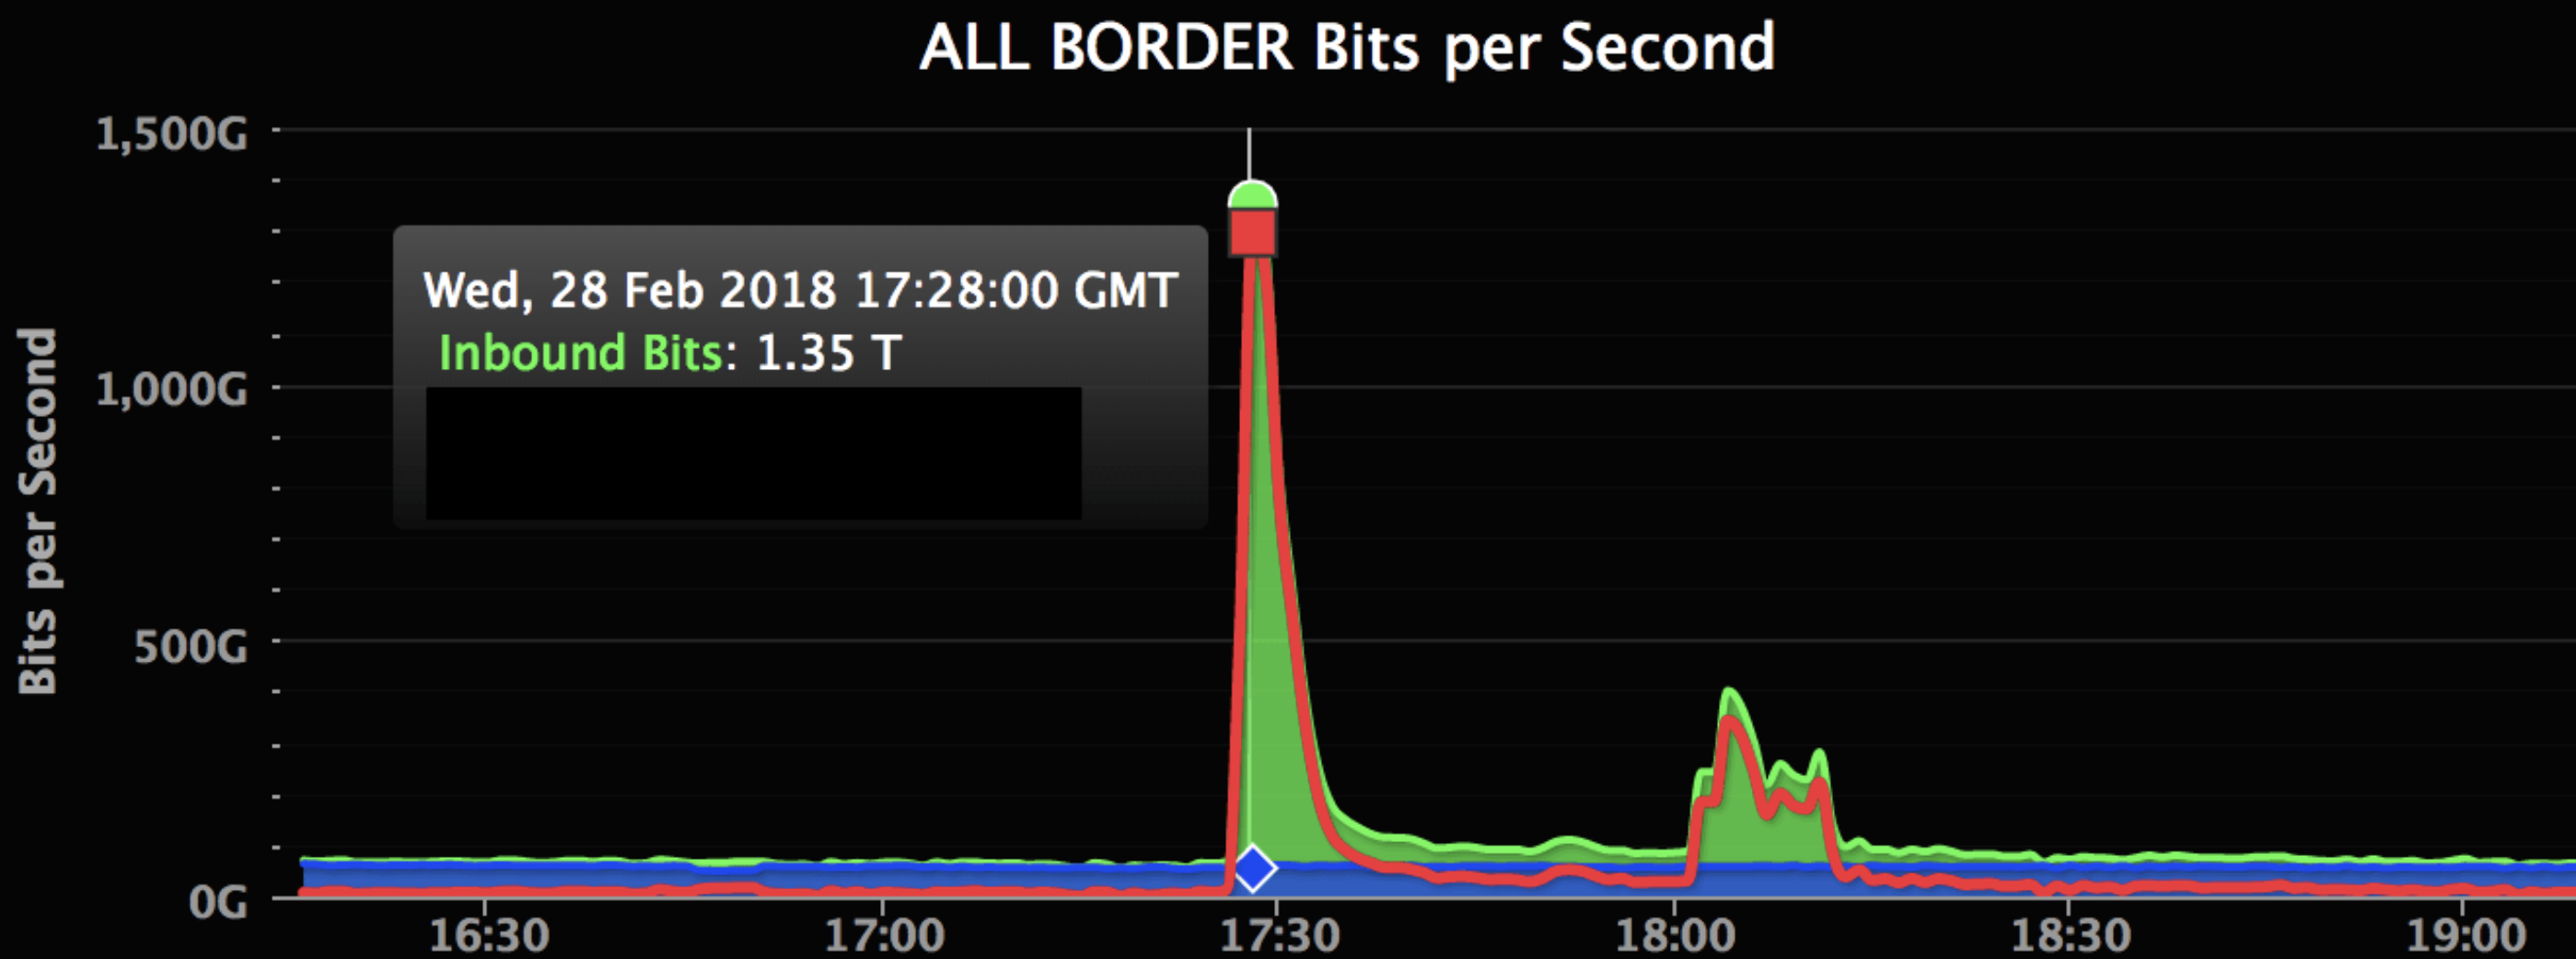
\includegraphics[scale=0.3]{Talk11/github} \end{center}
\caption{This graph provided by Akamai shows inbound traffic in bits per second that reached their edge. \textit{Quelle: https://github.blog/2018-03-01-ddos-incident-report/}}
\label{fig:github}
\end{figure}

	\subsection{DDoS Defense Systems}
		\subsubsection{Technical Solutions}
\textbf{\textit{a. Aggregate-based congestion control (ACC)}}

Mahajan et al. (2002) introduced two aggregate-based congestion control (ACC) mechanisms. The job of the first, local ACC is to identify the aggregates responsible for the congestion of a service and to throttle the throughput of these.

The identification of the offending aggregates is very difficult. The overload may be chronic due to an under-engineered network or unavoidable because the load shifted due to routing changes. The traffic might cluster in multiple dimensions (e.g. a particular server or network link) and the attacker may change their target to avoid detection.

The next challenge is to determine how much an aggregate should get throttled. The goal is to keep the service running during an attack, that implies they cannot block those aggregates completely. The rate limit is chosen so that the remaining traffic can at least maintain some level of service.

The second ACC mechanism is the pushback mechanism. The congested router pushes the aggregate throttling upstream to the adjacent routers sending him a significant fraction of the congesting traffic. This pushback propagates upstream to save bandwidth by dropping packets early and to focus on the routes or routers responsible for the congestion and still letting legitimate traffic through.

The pushback will not be effective against a DDoS attack, if the traffic is distributed evenly across the inbound connections. This can be possible, if the attacker uses an amplification (or reflector) attack with sufficiently distributed reflectors. Pushback can also overcompensate by throttling aggregates upstream that would not have been a problem downstream. Or if the pushback algorithm is not able to differentiate between malicious and legitimate traffic coming from the same edge network, that does not support the pushback mechanism. This fact could even be abused by blocking legitimate incoming traffic from a particular source by launching the attack from a host that is close to this source [11].

\textbf{\textit{b. Max-Min Fair Server-Centric Router Throttles}}

Yau et al. (2005) proposed and tested a router throttle mechanism that aims to increase the precision in blocking malicious and protecting legitimate traffic. This is a server-initiated proactive approach, where the server protects itself by installing a router throttle at an upstream router. The throttles depend on the current demand and have to be negotiated dynamically between server and network.

If a server load crosses the load limits, the server installs the throttle at some of its upstream routers. There is a defined upper and lower limit and if reached, the throttle rate is reduced further or increased again.

The fair throttle algorithm tries to minimize the throttling on well behaving routers, by not just decreasing the allowed traffic from every router, but by multicasting a uniform leaky bucket rate (i.e. the throttle rate) to all targeted routers. This way, busier routers drop much more packets then calm ones, which may not have to drop any [12].

\textbf{\textit{c. Probabilistic Packet Marking}}

Park and Lee (2001) discussed the effectiveness of IP traceback mechanisms based on probabilistic packet marking (PPM). The aim of probabilistic packet marking is to reduce the overhead produced by deterministic packet marking (DPM).In DPM, each router inscribes its local path information onto the passing packet. Those markings allow the destination node to trace back the traversed path of a packet but increases the packet header size linearly with every hop.

In PPM, the packet header provides a constant space for traceback information and after every hop, the router overwrites this information with a probability p < 1. This allows the destination node to trace back the whole path of the incoming packets, if the attack volume is high enough but also leaves the possibility open, that some packets still contain the original markings of the attacker, who can try to confuse the traceback.

In the case of DDoS attacks with a high number of attacking sources, this technique gets rendered more and more useless. The uncertainty grows more and more while the probability to find the sources becomes smaller and smaller [13].

\textbf{\textit{d. Hash-Based IP Traceback}}

Snoeren et al. (2001) present a hash-based IP traceback technique, that allows to trace back the origin of a single IP packet. They developed the Source Path Isolation Engine (SPIE). The engine enables to trace back a packet with a copy of the packet, its destination and an approximate reception time. The main goals of this technique is to reduce memory requirements and to not increase the vulnerability to eavesdropping of a network.

To achieve those goals, SPIE produces a 32-bit packet digest using a hash function. As hash input, it uses the invariant portion of the IP header and the first 8 bytes of the payload. Because it is not possible to store the digest of every packet forwarded on the router, SPIE uses a Bloom filter. This filter computes k distinct digests using k distinct hash functions. The hash function have to be uniform. The n-bit results get indexed to a bit array of the size 2n. If the copy of the file to trace back gets indexed to only 1-bits, with high possibility, the packet got forwarded by this router [14].

\textbf{\textit{e. Packet Filtering using Traffic Quota}}

The DDoS Defense System proposed by Xu and Lee (2003) assumes that the firewall is the bottleneck during a DDoS attack. The Server and Client do not need to be changed and the firewall issues the filtering operation. The goal is to produce a line of defense in the local network with a set of routers, typically belonging to a local ISP. Those so-called perimeter routers should distinguish between DDoS and legitimate traffic. They distinguish two types of DDoS attacks, the first where the attacker uses IP spoofing and the second where the legitimate IP addresses are used.

In the first case, if the first packet of a client arrives, the client gets redirected to a pseudo-IP address and port number pair. This new destination IP address contains a Massage Authentication Code (MAC) that's encrypted with a symmetric key shared between the firewall and the perimeter routers. If the senders IP address is spoofed, the HTTP redirect message will never reach him.
To avoid the collecting of valid MAC's from legitimate clients, the Key changes over time and gets a small timestamp or version number.

in the second case, where the attacker uses the real IP addresses, they cannot be distinguished from legitimate customers. The firewall has the job to allocate the available bandwidth fairly between all clients. Using a Deficit Round Robin algorithm, every client gets a traffic quota and all excess packets are dropped. The firewall tracks the amount of dropped packets and blacklists clients overreaching a particular threshold. To defend against a continuous attack that stays in the traffic quota, a "no loitering" law is enforced. If the total amount of packets sent by a client is bigger than a given quota, its traffic quota gets reduced to a fraction.

The main problems are, that a IP spoofed DDoS attack can make it hard for legitimate clients to get their first package through to get redirected and if all attackers use their fair share using genuine IP address, the service can suffer a response time too big for real customers to deal with [15].

\textbf{\textit{f. Hop-count Filering}}

Jin et al. (2003) propose a hop-count-based approach to filter out spoofed IP packets. They use a victim-based approach that does not need the support of the ISP's. The only information needed is contained in the package header, assuming that in most cases of IP spoofing the hop-count of the package does not correspond to the expected hop-count of the IP address. The hop-count can be inferred from the TTL field of the incoming packets. To avoid dropping packets of legitimate clients because the hop-count information is not correct, the filtering only takes place if an attack gets detected [16]. 

		\subsubsection{Economic DDoS Defense (Honeypots)}
Defending against DDoS attacks with technical solutions results in an arms race between attacker and defender. It has become more common to not only look at technical solutions against direct DDoS attacks, but to target the economic aspects of botnets.

Ford and Gordon (2006) describe their Multihost Adware Revenue Killer (MARK), to attack the revenue streams of botnets used for unwanted advertisement and software installs on the victim's machine (Adware and Spyware). This use of botnets is thought to be the most profitable for botmasters. MARK consists of Virtual Machines (VMs) which actively try to get infected by Ad- and Spyware, so called honeypots. Because no one sees the ads shown on those VMs and there is no personal information to find, the botmaster's revenue increases first, but the advertisement or spyware distributer loses money. This destabilization can lead to a massive decrease in payment (i.e. per click or per download), and therefore a massive decrease in revenue for the botmaster when the VMs get cleared and the honeypots are no longer generating revenue [17].

Li et al. (2009) propose a similar strategy, with the goal to make it more troublesome for botmasters to maintain their botnets. They focus more on DDoS attacks and propose to use honeypots to introduce uncertainties to the optimizing problem of botmasters and clients. The honeypots do not participate in DDoS attacks, for this reason the required number of bots for a successful attack increases and the value of a single bot decreases by consistent maintenance costs. According to their model the profits of attackers and botmasters can decrease dramatically [2].

\section{Economics}
	\subsection{Introduction}
	As a subset of the cybercrime economy, the botnet economy plays out on underground black markets. Over time there has been a shift in incentives, where the attackers are no longer motivated by self-fulfillment and proof of skill, but rather the financial gain attributed to such attacks. (Li et al. "Botnet economics: Uncertainty matters") As part of this shift towards economic incentives, cybercriminals have developed business models that shall guarantee the profitability of their botnets. (Li et al. "Botnet economics: Uncertainty matters")

The many victims affected by botnets are faced with a serious economic threat. Successful DDoS attacks on companies may lead to both direct economic costs, as well as indirect losses which are much harder to quantify. Direct costs occur due lost revenue during the server's downtime. Indirect losses measure the long-term effect loss of customers trust and market share have on revenues. The value destroyed by these attacks also inflict costs on society at large. The damages, although difficult to quantify, are estimated to be in the tens of billions of dollars every year. (H. Asghari et al. "Economics of fighting botnets: Lessons from a decade of mitigation")
This chapter shall give an overview of the different stakeholders involved, the business models used to operate successful botnets, as well as an attempt to model the different types of economic damage a botnet attack can inflict. 

	\subsection{Stakeholders}
			In order to gain a better perspective on incentives and the botnet economy as a whole, we first have to define the relevant partners effected by botnets. We will analyze both the parties involved on the attacker and the victim sides.
			
		\subsubsection{Attackers}

			The following is a list of key partners involved on the side of the attacker. We based this list on papers written by C.G.J. Putman et al. "Business Model of a Botnet" and G. Bottazzi et al. "The Botnet Revenue Model".

			\textbf{\textit{a. Malware Developers}}
			
			Malware Developers are mainly IT professionals involved in the research and development stage of the botnet life cycle. They identify vulnerabilities in software, develop new malicious software to exploit these vulnerabilities, and maintain existing software. No illegal activities take place in this step of R\&D. Only the use of the software is considered illegal.

			\textbf{\textit{b. Money Handlers}}
			
			The goal of money handlers is to offer payment services with a high degree of anonymity. They allow people buying malicious software to remain anonymous. The malware developers from the first stage also have an interest in remaining unidentifiable, as to not be charged as an accessory to any crimes committed by the buyer. The supply of anonymous payment services is also not considered illegal and can be achieved through the use of cryptocurrencies.

			\textbf{\textit{c. Command and Control Bulletproof Hosting Providers}}
			
			Bulletproof Hosting allows the botnet end-user to store any stolen information such as passwords, banking accounts, or other credentials. The control center for the botnet, which can also be provided through the hosting service, consists of one or multiple computers.

			\textbf{\textit{d. PPI (Pay Per Install) Distributors}}
			
			The distribution and multiplication of malicious software is constantly evolving, and many developers lack the necessary resources to spread their malware effectively. For this purpose, developers use a PPI model, which essentially allows them to spread their software by commissioning third parties with the infection and paying them a certain fee per infected device. According to research by Brian Krebs proposed in his paper "Most Malware Tied to Pay-Per-Install Market", PPI costs are estimated to vary from \$7 to \$180 per 1000 installations.

			\textbf{\textit{e. Botnet Owners}}
			
	Botnet owners, also known as botmasters, are the ones who actually perform the attacks. They either perform these malicious activities for their own personal benefit, or on the behalf of third-party users for financial gain. The latter is the becoming more common according to Li et al. in their paper "Botnet Economics: Uncertainty Matters".

			\textbf{\textit{f. Botnet Users}}
			
			Botnet users are the final piece in the botnet supply chain. They are customers willing to pay money to make use of the botnet and perform attacks. Users are mainly charged by the pay-per-use model.

The figure below provides an overview of different stages of the botnet life cycle and the parties involved. 


\begin{figure}[ht]
\begin{center} 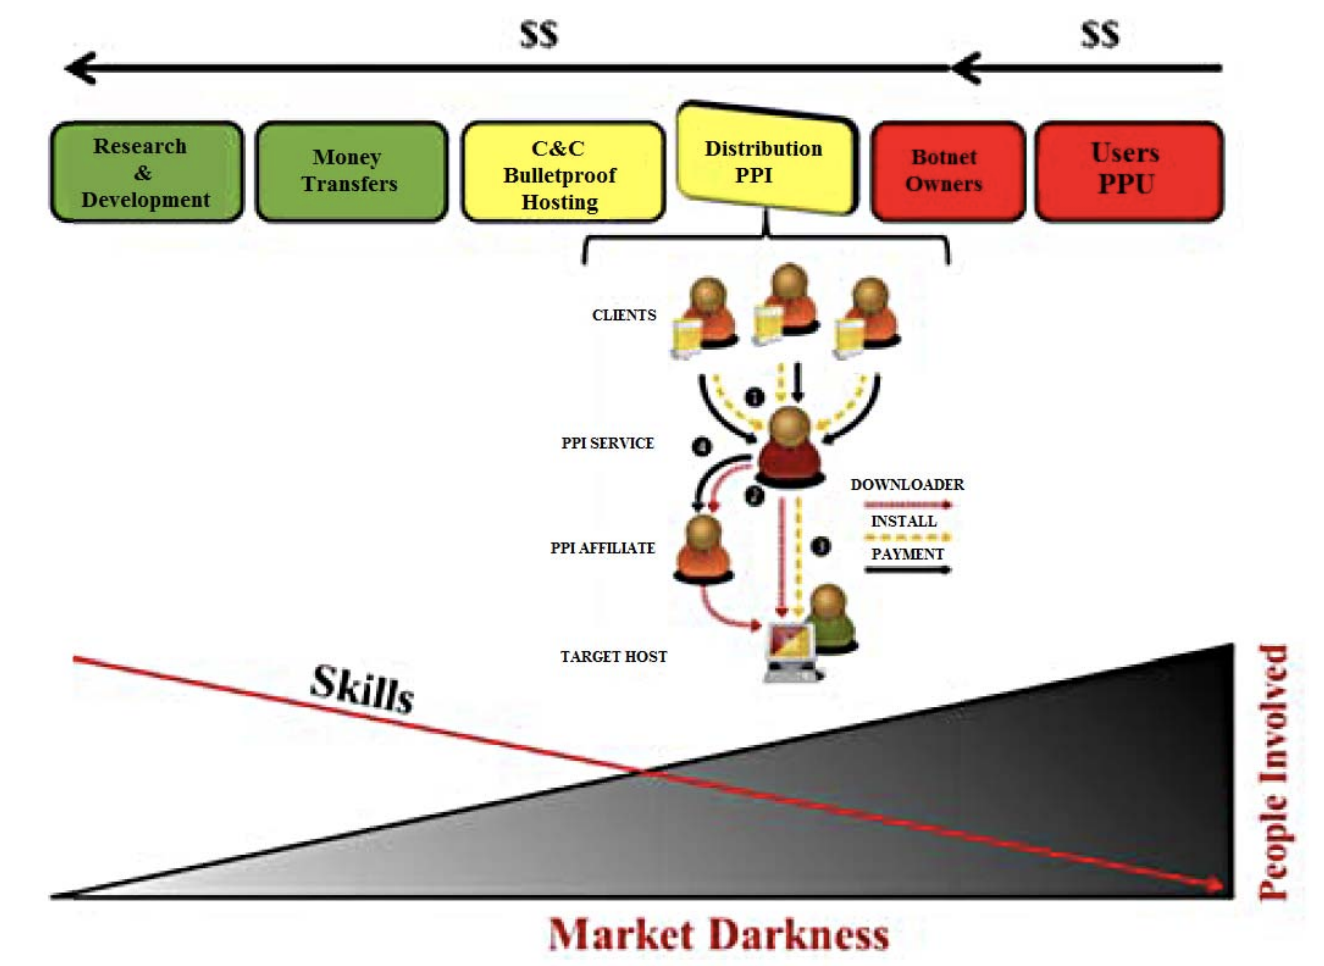
\includegraphics[scale=0.6]{Talk11/RevenueModel} \end{center}
\caption{The Botnet Revenue Model}
\label{label}
\end{figure}

		\subsubsection{Victims and Defenders}
	The following is a list of victims affected by botnet attacks and third parties involved in defensive measures, as well as their incentives to protect themselves from these attacks.

			\textbf{\textit{a. Victims of DDoS and Spamming}}
			
			The first and probably most obvious victims are the ones that suffer from DDos attacks and spamming carried out by botnets. The victims of such attacks suffer far-reaching financial consequences from such attacks. Oftentimes, the targets are businesses who suffer direct losses in the form of lost revenue due to the unavailability of their online services. But they also suffer indirect impacts, such as a loss of customer trust and market value. These damages are usually far more severe (Anderson et al. in "Measuring the cost of cybercrime") and harder to quantify due to the difficulty of attributing these losses directly to botnet attacks. As a result, businesses with a certain exposure to malicious attacks and a strong reliance on online presence, have very strong incentives to protect themselves from botnet attacks. Additionally, the loss of customer trust and market shares that these attacks entail, lead companies to try and keep information about suffered attacks out of the public eye.

			\textbf{\textit{b. End-users of Infected Devices}}
			
			Another obvious direct victim are the end-users of the infected devices. In the case of DDos and spamming attacks, the users of infected devices are not directly affected by any negative consequences, as they are simply used as a means to an end. Therefore, they may lack certain incentives to protect themselves adequately from malware and not become part of a larger botnet. (Asghari et al. "Economics of fighting botnets: Lessons from a decade of mitigation") Why should a device owner pay for security measures, when he does not suffer any direct economic consequences from being infected? Another explanation might be that many end-users are simply not aware of the danger malware entails and therefore lack the knowledge required to adequately protect themselves from such attacks.

Other forms of botnet attacks, such as identity and information theft, bank fraud, and phishing, do however pose a direct threat to owners of infected devices. According to an estimation by Anderson et al. in "Measuring the cost of cybercrime", consumers globally suffer losses in the range of \$70 million due to online banking fraud. For business, that number rises to around \$300 million. Furthermore, Anderson et al. estimate that global expenditure on antivirus protection reached \$3.4 billion in 2012. While the indirect cost for users for the clean-up of malware in the same year is estimated to be around \$10 billion globally and \$500 million in the UK alone.

			\textbf{\textit{c. Antivirus Software Vendors}}
			
		As mentioned in the section above, security vendors have very strong financial incentives to provide protection from malicious software, as the global expenditure is estimated to be around \$3.4 billion any a large majority of consumers have some sort of antivirus software. Additionally, global expenditure on clean-up is estimated at \$10 billion and therefore provides even more financial motivation for security vendors. (Anderson et al. in "Measuring the cost of cybercrime ")

At this point however, it has to be state that this includes cost for protection against malware in general and not only related to botnet attacks. Vendors of such software are also faced with large development and maintenance costs, as cybercriminals constantly try to find new ways of circumventing existing protection measures.

			\textbf{\textit{d. Internet Service Providers}}
			
		Internet Sevice Providers (ISPs) play a large role in botnet mitigation, as they are able to perform measures on a very large scale and therefore more economically that single end-users. They do however lack accountability, as they are not the cause of botnets, and economic motivators, as such counter measure can be very costly, and ISPs do not suffer any direct consequences by users being affected by cybercrime. Advanced detection and follow up actions can also cause privacy concerns of customer data. (Pijpker et al. " The Role of Internet Service Providers in Botnet Mitigation ")

Still internet service providers do play a role in botnet mitigation due to organizational and institutional incentives. " Relevant organizational factors for ISPs to address botnet mitigation include the size of their customer base, the internal organization of their abuse desk, and the cost spend on various security measures. " (Pijpker et al. " The Role of Internet Service Providers in Botnet Mitigation ") Institutional incentives on the other hand are not imposed internally, but rather by policy makers and market conditions. They include for example the regulatory context and market settings. (Pijpker et al. "The Role of Internet Service Providers in Botnet Mitigation ")

Research shows that ISPs currently focus more on prevention and notification of customers and that there is still quite a lot of room for improvement due to a lock of incentives for botnet detection, remediation, and recovery on the behalf of internet service providers. (Pijpker et al. " The Role of Internet Service Providers in Botnet Mitigation ")

			\textbf{\textit{e. Law Enforcement}}
			
		As costs for cybercrime mitigation can be very high, additional investments in law enforcement can be an effective counter measure. The cost for law enforcement is generated by the time required to find and prosecute cyber criminals [10]. Anderson et al. estimate that the global expenditure on law enforcement for cyber crime defense is around \$400 million, while that of the UK is about \$15 million in 2010 [10]. When compared to the cost of cybercriminal infrastructure of private corporations, this modest number may be one reason for the low success rate in finding and punishing cyber criminals. 
		
	\subsection{Revenue Streams and Incentives for Botnet Owners}
		Even though botmasters are not always solely financially motivated, there are several potential revenue streams for botnet owners. The following chapter shall provide a non-extensive list of possible revenue streams for botnet owners with some estimations on the revenue they generate. The following figure provides an overview of all the different revenue streams mentioned in this chapter.
		
		
\begin{figure}[ht]
\begin{center} 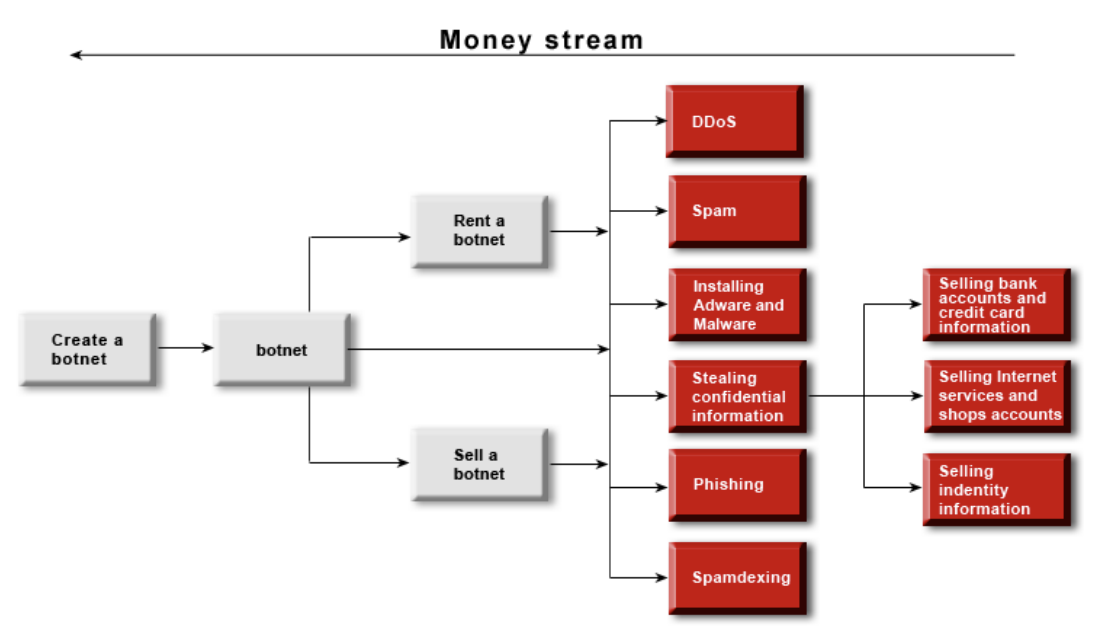
\includegraphics[scale=0.6]{Talk11/RevenueStreams} \end{center}
\caption{Botnet Revenue Streams}
\label{label}
\end{figure}
		
		\subsubsection{DDoS Attacks}
		DDoS attacks are one of the most common malicious activities performed with the use of botnets that can be highly lucrative. The goal of a DDoS attack is to force a computer system into denial of service for legitimate customers by sending enough requests to the computer of a victim that it can no longer process all of them [1]. Two possible revenue streams can be implemented for DDoS attacks.

The first of which is extortion [4]. Owners of botnets can generate profits with simply threatening to perform a cyber-attack. Oftentimes large companies give in to such demands due to the immense costs associated with a successful DDoS attack, both direct and indirect [1].

Additionally, botnet owners can offer their services in underground forums in the form of a DDoS-for-hire service which operate on a subscription or pay per use basis. Prices for single DDoS attacks vary largely on the number of bots needed to perform the attack. They can range from only about \$50 for an attack on a small unprotected online store to several thousand dollars for attacks on large international companies who have well protected web sites. This makes sense, as the cost of operating a botnet increases immensely with higher number of devices controlled by the botnet. [1] Subscriptions allow users to manually perform an unlimited or limited number attacks any time they would like through front-end web servers. Prices for these subscriptions vary from just \$5 up to \$300 dollars and allow customers to use the service for one to three months, depending on the tier of the subscription [4].

One example of such a booter service is VDoS. VDoS generated revenue in the region of \$25,985 per month over the course of two years of operation, with their lowest performing month at \$9,956 and their best performing moth at \$42,924 [4]. As they are almost impossible to quantify, there is no information on profits generated from extortion [1].

		\subsubsection{Information Theft}
		Another source of revenue for botnet owners is the sale and misuse of personal information such as bank accounts and credit card information, online credentials, or identity information. This type of data is directly extracted from the infected bots [2]. Cybercriminals can decide whether they want to use the gathered information for their own use or sell them to third parties. The price for a bank account can range between \$1 and \$1,500. The low value of this information can be attributed to strong competition from other vendors. In order to generate a lucrative and sustainable revenue stream, botmasters constantly need an inflow of new data and a large botnet [1].

One example that shows how lucrative bank account theft can be is the case of Eurograbber. In an attack on European online banking customers through a Zeus based mobile trojan, the perpetrators were able to illicitly transfer funds over 36 million Euros from more than 30,000 bank customers. [3]

		\subsubsection{Phishing}
		In order to protect phishing sites from being shut down and extend their lifetime, cybercriminals are offering an implementation of fast flux technology, which allows phishers to change their website's IP address every few minutes without altering the domain name. This technique of using infected home computers as web servers with phishing content also makes them harder to track down. [1]

In order to acquire a ready-made botnet for their fast flux solution, phishers pay botnet owners \$1,000 to \$2,000 per month. The average income and damage to consumers is in the millions of dollars per year and comparable to that from theft of personal information. [1]

		\subsubsection{Spam}
		One of the most important applications for botnets is sending spam. Spammers use different business models; some make profits by luring users to infected websites where they might download malware while others are part of phishing campaigns designed to steal user credentials for reasons mentioned above. Botnets provide the required infrastructure necessary for carrying out spamming services. [5]

Prices for spamming services depend on the size of the target audience and can range from just \$70 for a few thousand addresses up to \$1,000 for tens of millions of addresses. [1] In their paper " The Economics of Spam " Justin Rao and David Riley estimate that American firms and consumers experience costs of about \$20 billion per year due to spam messages. Furthermore, they estimate that spammers and spam-advertised merchants make revenues of about \$200 million worldwide annually. This means that the externalities caused by spam messages has a ration of 100:1. [6]

		\subsubsection{Spamdexing}
		Spamdexing, also known as search engine spam, are a form of deliberate manipulation of search engine indexes to improve a website's position in search engine results. The idea behind this is that websites with a higher position generate more clicks and therefore revenue. 

There are several criteria search engines use to judge the relevance of a website for a given search input. The number of links to that particular website on other websites is one of the main factors in determining which result is displayed at the top. Botnets are used to create many posts and comments containing the link to websites being promoted and related keywords. The price for such services averages at about \$300 per month. [1]

		\subsubsection{Adware and Malware Installation}
		An additional revenue stream for botnet owners can be the installation of adware on infected computers. Adware is software that generates revenue for its creator by automatically and unwantedly displays advertisements in the user's interface, most often a web browser [7]. Companies that offer such adware often pay between 30 cents and \$1.50 for the installation. With thousands of computers at their fingertips the installation of adware and other forms of malware can be a lucrative and simple way to generate additional profits for botnet owners. A famous example is John Kenneth Schiefer, a hacker convicted in 2007 that used a botnet to distribute adware and managed to generate profits of around \$14'000 in one month. [1]

The pay-per-install business model is also used by cybercriminals when distributing malware. The average price for an installation varies depending on the geographical location of the computer, as an infected computer in developed countries are capable of generating a lot more profit because the information is oftentimes more valuable. The price for 1,000 installs in the United States for example can reach up to \$120, while the same number of installs on Chinese computers of generates about \$3 in profits. [1]

		\subsubsection{Cyber Fraud}
		Cyber fraud has many different forms. One very common form is click fraud, where websites and botnet owners generate profits from clicks on advertisements. This type of click fraud relies on pay-per-click advertising where companies that place advertisements on other websites, through Google AdSense for example, pay for these ads based on the number of clicks that they receive. A clickbot helps an attacker commit click fraud by generating fake clicks on ads. This technology can be used in a few different ways. For example, a company can generate a lot of clicks on the ad of a competitor in order to diminish their budget and create more costs. Alternatively, websites that publish the advertisements can also use clickbots to click on the ads placed on their own websites, as they receive a share of the profit from ad clicks. [8] Botnets allow attackers to generate thousands of clicks per day, all from different computers as to not raise any suspicions [1]. By analyzing Clickbot.A, N. Dawasi and M. Stoppelman estimated that Google can lose around \$50,000 with botnet of 100,000 bots. A share of this profit generated by advertisers then goes to the botnet owners. [8] Another click fraud botnet, ZeroAccess, has generated ad losses up to \$900,000 daily with 140 million clicks a day [2].

Another way to commit cyber fraud is by creating fake user ratings and customer reviews on websites or with the rising importance of cryptocurrencies, botnet owners can abuse the computing power of their botnets to mine cryptocurrencies [9].
		
\section{Case Study: Mirai}
	\subsection{Scenario}
	On October 21, 2016 there was a series of DDoS attack, which exceeded traffic of 1.3 terabytes per second on the popular Domain Service Provider (DNS) Dyn, which disrupted the name resolution for their clients. Services affected by the attack were high traffic sites, such as Amazon, Reddit, Spotify, Tumblr and Twitter. During the time of the attack internet users reported, that they had troubles accessing the affected websites for several hours. The attack was believed to be caused by Mirai, a botnet exploiting security weaknesses in IoT devices.
	
		\subsubsection{Timeline}
		According to the post-mortem report of Dyn, the first set of attacks started at 11:10 UTC. It was carried out with high-volume floods of TCP and UDP packets, both with destination port 53 from a very large number of source IP addresses. The Engineering and Network Operations teams of Dyn deployed additional mitigation tactics in addition to their automated response techniques, such as traffic-shaping incoming traffic, rebalancing of that traffic by manipulation of anycast policies, application of internal filtering and deployment of scrubbing services. At 13:20 UTC these mitigation tactics were fully in deployment and the services were restored.
		
Followed by that a more globally distributed set of attacks started at 15:50 UTC. Since this second set of attack used the same protocol as the first attack, Dyn could mitigate the attack for the most part by 17:00 UTC.
 
In addition to the attacks on Dyn, there were simultaneous attacks on Xbox Live, Microsoft DNS infrastructure, Playstation, Nuclear Fallout game hosting servers and Valve Steam servers. At 22:17 UTC, the final 10-hour long attack was issued on a set of Dyn and Playstation infrastructure. This suggests that the attacker was targeting gaming infrastructure and the attacks on Dyn were collateral damage. Cloudflare also came to this conclusion, as the other targets attacked DYN variant were all related to providing services for videogames.

In the following days numerous smaller TCP attack occurred, which were mitigated by the efforts of Dyn and left their customers with no signs of disturbance.
"There was a 71\% intersection noted in a study between the 107K IP addresses spotted that attacked Dyn and the Mirai scanning in their network telescope. They concluded that while Mirai was clearly involved in the attack, there may have been other hosts involved as well."

		\subsubsection{Motives}
		Two days after the attack the New York Times stated that investigators suggested that the attack was either conducted by a criminal group that wanted to extort the company or were motivated by hacktivism. They also mentioned the possibility of a foreign power, which wanted to remind the United States of its vulnerability.
In January 2017 a post was released on the internet security blog Krebs on Security by, which disclosed the supposed name of the author of the Mirai Botnet Paras Jha, a 22-year-old student of Rutgers University. Jha publicly released the source code of the Mirai botnet on an infamous public internet forum "HackForums" under the name "Anna-Senpai" on September 30. 

Following investigation and questioning by the FBI Paras Jha, Josiah White and Dalton Norman entered a guilty plea in December 2017. Jha was fined \$8.6 million and sentenced to 2'500 hours of community service for using Mirai to attack the computer system of his university.

Paras Jha admitted to investigators that he launched his attacks on the computer system of Rutgers University not out of financial gain, but for other personal motivations. The first attack he launched, was for delaying registration upper-class men registration to an advanced computer science attack he wanted to take, whereas the second attack was to delay an exam. Other attacks on the computer system were launched for his personal amusement to see outrage.

Furthermore botnets similar to Mirai or early prototypes were already in use as early as 2014 by a group of hackers going by the name of "lelddos", which targeted Web servers hosting Minecraft, a very popular sandbox video game, where you can build your own world with other players in a blocky realm. The Minecraft server hosting market is very competitive, and a very successful server owner can make over 50'000 USD per month from renting space for players to build their world. Lelddos has targeted these lucrative Minecraft servers for years with their attacks and extortion attempts. 

Jha nor his fellow co-authors admitted any involvement in the Dyn attack and even to this day it's unknown who the perpetrators behind the cyberattack on Dyn were. A group called "New World Hackers" claimed responsibility shortly after the attack. Other groups such as Anonymous and SpainSquad declared that they were the perpetrators behind the attack but none of the claims were confirmed.

The facts that the targeted services were associated with gaming and Jha's personal use of the botnet suggests that there was no personal financial gain as a motive behind the Dyn attack, but it served as an act of internet vandalism.


	\subsection{Business Model}
		\subsubsection{Operation}
		Unlike many other botnets Mirai primarily targets Internet-of-Things (IoT) devices running on ARC processors, such as IP cameras and home routers. In a first step Mirai enters a rapid scanning stage where it aimlessly sends out TCP SYN probes to to pseudo-random IPv4 addresses on Telnet TCP ports 23 and 2323, excluding those in addresses in a hard-coded blacklist. On recognizing a potential victim, Mirai then tries to log into the device with a brute force attack using 10 randomly selected username and password combinations out of a list of 62 common factory default usernames and passwords (e. g. 'admin' \& password).
		
After a successful login various characteristic are sent to a report server through a different port. These reports are used by a C\&C server to continually determine new prospective victims. This server also communicates with the report server to get the current status.

The botmaster then sends an infect command in a separate loader program with the necessary details, such as IP address, system environment and hardware architecture. A separate loader program then logs into the target device and gets it to download the corresponding binary, usually via GNU Wget or using FTP (File Transfer Protocol). 

The loader then executes the corresponding binary version of the malware on the device. If the execution of the malware was successful it is stored in the RAM of the device. Due to this fact, a reboot of the device will remove the malware. At this point Mirai is ready for further instructions from the botmaster while continually scanning the environment for prospective targets.

Additionally, Mirai attempts to conceal its presence by removing the downloaded binary and change its process name to a pseudorandom alphanumeric string. Furthermore, access points such as telnet or SSH services are shut down to protect itself from other Malware. In another step Mirai attempts to conceal its presence by removing the downloaded binary and changeing its process name to a pseudorandom alphanumeric string.

Besides this point Mirai does not care about the footprint it leaves behind, relying on the fact that IoT devices have very loose security in comparison to the likes of personal computers. Every stage of infection is recognizable by signatures such as sequentially testing specific credentials in specific port during the brute force access phase or sending reports with distinctive pattern to the report server.

During a DDoS attack the infected devices receive an attack command by a C\&C server and only must resolve a hardcoded domain name in the executable of the malware. This leads to a lower need for communication as the botmaster can choose another target IP address without changing the binary and additional communication.
Mirai makes use of 10 different attack methods, which can be distinguished within four categories:

In the attack on Dyn most of the attacks used were SYN floods on the DNS port 53 with few GRE IP attacks. Additionally, the attacks on the gaming services, mostly Playstation Networks infrastructure were carried out via ACK and GRE IP floods with VSE suggesting that another target were the Valve Steam Servers.

	\subsubsection{Costs}
	In a case study in 2016 regarding the Mirai Botnet it was mentioned that the costs of maintaining desktop botnets exceeds the revenue from DDoS attacks for most botnets. Due to the technological advance in anti-DDoS services, DDoS protection are more affordable than they used to be, which leads to the decline of ransom-driven DDoS attacks.
	
The maintenance of a botnet consisting of IoT devices is more lucrative, which Mirai takes advantage of. Although rebooting would remove the malware, only changing the password or more drastic measures would remove the risk of reinfection. Furthermore, users generally have little control over IoT devices, which makes them only more attractive of a target. These factors lead to reinfection being very likely to succeed for the maintainer of a botnet.

A person controlling the botnet only must keep a list of the IP addresses, which have been infected in the past, and scan if they're still connected to the botnet. The cost for reinfection has been estimated to be at \$0.0935 per device. In addition to that there are additional costs, such as keeping the software updated in the arms race between hackers and defenders.
Also, the costs are estimated to be around \$7 to \$180 per 1'000 installations (\$0.007 to \$0.18 per device). Furthermore, the cost for spreading is estimated to be at around \$0,016 per device.

According to a case study of Charlie Miller, a level 1 malware develop earns around \$125k a year. Based on this estimation and under the assumption that the developer works 8 hours a day and 22 days in a month, the cost of maintaining a botnet can be estimated to be \$59 per hour.
From the conclusion of another study they concluded that the initial investment such as acquiring and spreading the malware and the recurring costs are nearly insignificant compared to the revenue it makes. Furthermore, there was noted that out of three of four case studies, the set-up costs for a botnet accounted to a maximum of 1,1\% of the found monthly revenue.

	\subsubsection{Revenue}
	Although the \$59 per hour stated in the last section might seem costly, advertising and renting out a botnet costs little if no money. The hacker Popopret gave an example of the cost of renting out a modern variation of the Mirai botnet. A botnet attack of 50'000 bots with an attack duration of 1 hour and a 5-10-minute cooldown goes for roughly 3-4k per two weeks. This botnet is controllable through a console on the Tor network and can be accessed via telnet.
	
In addition, the Mirai botnet was also used by Jha and Norman to commit advertising fraud, including click fraud as a less noticeable way to generate passive income by abusing pay-per-click online advertising sytems with more than 100'000 infected devices.

IBM X-Force researchers found out that some modern variations of the Mirai botnet were also using the computation power of infected devices to mine cryptocurrency. Although this kind of usage is more noticeable in the IoT devices as it could damage by overheating the devices little central processing and graphical processing unit resources.

	\subsection{Economic Impact}
	In February 2017 data was published by security services company Bitsight, which showed that Dyn lost a considerable number of customers after the incident. Dyn lost business of about 8\% of their domains, about 14'500 shortly after the attack of their total 178'000, which were analyzed by Bitsight. 
The biggest loss was spotted in websites, which used Dyn and another DNS provider. About 8'000 domains were lost, 24\% of this category of websites. Websites which used Dyn exclusively as a DNS provider mostly continued to use Dyn, only losing 4\% or around 6'000 websites. Bitsight stated though that there is no indication if any of the lost customers went back to Dyn after the attack as it was only a snapshot of the monitored websites.
Furthermore, the experienced inaccessibility caused a lot of damage for the involved websites. 

Estimating the loss for Amazon would be with their reported profit of almost 136 billion USD in 2016 would be around \$260'000 per minute. Assuming the downtime was around 3 hours, the estimated damage adds up to 46 million during this timeframe. With other affected internet giants, the damage dealt in the Dyn attack is in the region of multiple hundred million, if not billions.

	\subsection{Aftermath}
	The Dyn attack as the biggest DDoS attack until the attack on GitHub in 2018 brought the spotlight to Mirai to the media in masses and highlighted the vulnerabilities of IoT devices and the importance of investing into DDoS protection services. It served as a wake-up call to many IoT manufacturers. Matthew Prince, the CEO of Cloudflare, a popular DDoS protection service stated that various IoT manufacturers asked the sales team for help to protect against attacks. Especially companies manufacturing IoT devices, where the malfunctioning of the devices could have serious implications, such as in the automobile or healthcare industries, were especially concerned.
	
Since Jha releasing the source code of Mirai back in 2017 there have been many copycats using modern variations of the Mirai botnet even to this day, increasing the number of C\&C servers by a large amount. Due to this fact, it has been more difficult to track down the origins of attacks of mirai-like botnets nowadays.
Mirai experienced a resurgence in 2019 with a focus-shift in targeting enterprise environments due to a greater number of devices than in households. In enterprise environment many of the targets (more than 80\%) are in the media/information services or insurance industries.

Whereas there were around 15 billion connected IoT devices in 2016, forecasts estimate that this number will exceed the 20 billion mark in 2019. In a Securelist report it was estimated that about 21\% of IoT device infections in 2018 were carried out by Mirai-clones.



\section{Evaluation and Discussion}
Text

\section{Summary}
Text
